\documentclass[12pt,a4paper,titlepage,spanish]{article} 
\usepackage{babel}
\usepackage [T1]{fontenc}
\usepackage [latin1]{inputenc}
\usepackage{graphicx}
\usepackage{amssymb}
\usepackage{amsmath}
\usepackage{setspace}
\usepackage{epsfig}
\usepackage{enumerate}
\usepackage{float}
\usepackage{array}
\usepackage{cancel}
%\usepackage{arcs}
\usepackage[usenames,dvipsnames]{color}
	  \oddsidemargin 0in
      \textwidth 6.75in
      \topmargin 0in
      \textheight 10.0in
      \parindent 0em
      \parskip 2ex
\usepackage{anysize}
\marginsize{3cm}{2cm}{1.0cm}{1.0cm}
\pagestyle{plain}
\title{
\begin{Large}
 \begin{center}
		\underline{Informe Simulaciones TP11: M�todo de rechazo} \\
		\underline{Generaci�n de n�meros aleatorios con distribuciones no uniformes}\\
		\underline{Curso: } 6to 1ra\\
		\underline{Turno: } Noche\\
		\underline{CPU: } Intel Core 2 Duo E6600\\
      \end{center}
\end{Large}
}
\author{Vileri�o, Silvio}

\begin{document}
\maketitle
\setcounter{page}{2}
\tableofcontents
\newpage

\subsection{Introducci�n}
En esta simulaci�n se utiliza el m�todo de rechazo para generar n�meros aleatorios con distribuci�n no uniforme. Este m�todo, a diferencia del anterior (Transformada Inversa), permite hallar funciones distribuci�n no integrables anal�ticamente,
o funciones trascendenales (funciones donde no se puede despejar la $ X $ como por ejemplo $ x^2 = \cos X $ ).

\begin{equation*}
	\\Sea\left\lbrace
	  \begin{array}{l}
		\text{$ f(x) $ una funci�n definida en el intervalo } [ \alpha, \beta ] \\
		\text{$ x $ } \in \mathbb{R_a}  [ \alpha, \beta ]\\
	  \end{array}
	  \right.
\end{equation*}
Se desean generar $ K $ n�meros aleatorios donde $ \alpha=1 $ , $ \beta=10 $ dando un intervalo $ [1, 10] $ con una funci�n de distribuci�n o reparto del tipo $ f(x)=\frac{1}{x} $, de forma que la distribuci�n quede dada por $ f(x) $ y el
histograma adquiera la siguiente forma:\\
\begin{center}
	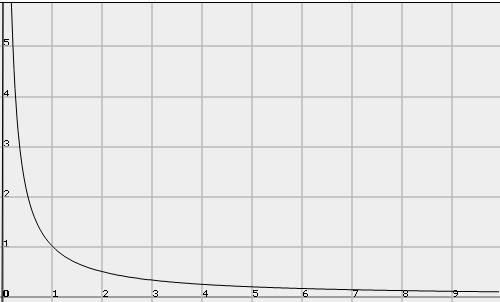
\includegraphics[scale=0.75]{images/Distribucion-1x.JPG}
\end{center}

Se procede a calcular $ N $, que indica la cantidad de puntos en un intervalo(estad�sticamente).
\begin{center}
 $ N=\int_\alpha^{\beta}\frac{1}{x} \: dx $
\end{center} 
Una vez calculado $ N $, se calcula la funci�n normalizada $ g(x)=\frac{f(x)}{N} $, la cual nos d� la probabilidad de aparicion de x.
El m�todo de rechazo consiste en la generaci�n de un n�mero al azar en un intervalo $ [\alpha, \beta] $ y adem�s, la generaci�n de un discriminante en el intervalo $ [0,1] $, que servir� como ruleta para la selecci�n de los n�meros aleatorios.
Si $ Rnd\leq g(x) $, el n�mero es contado como v�lido, de no ser as�, se repite la operaci�n hasta lograr $ K $ n�meros. En este caso, se pide llevar una cuenta, de n�meros generados, n�meros admitidos y n�meros rechazados.

Funci�n $ g(x) $
\begin{center}
\textcolor{green}{$ y=\frac{1}{ \log(\beta) . x} $}
\end{center}
Luego de realizar la simulaci�n, se obtuvieron los siguientes resultados: \\
\begin{itemize}
	\item Funcion $ f(x)=\frac{1}{x} $
	\item Intervalo $ [1, 10] $
	\item	Total Numeros Generados: 9007211
	\item Total Numeros Admitidos: 1000000
	\item Total Numeros Rechazados: 8007211
\end{itemize}
\begin{center}
	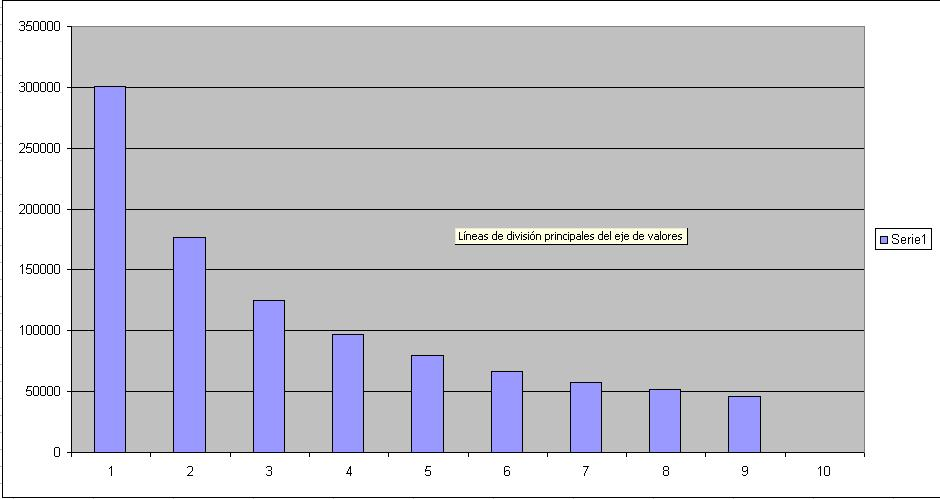
\includegraphics[scale=0.50]{images/Histograma.jpg}
\end{center}
\newpage
\subsection{Conclusi�n}
Se comprueba que por medio de este m�todo se pueden obtener distribuciones en funci�n de una transformada cualquiera, \underline{sin importar si la funci�n no es integrable anal�ticamente} \\
\underline{ y/o trasncendental}, en este caso se pide la funci�n $ f(x)=\frac{1}{x} $. Es un m�todo efectivo, pero en comparaci�n con el m�todo de la transformada inversa, solo deber�a utilizarse cuando realmente es necesario, ya que el costo computacional es casi 10 veces mayor. 
\end{document}